\documentclass[a4paper,12pt]{article}
\usepackage[latin1]{inputenc}
\usepackage[T1]{fontenc}
\usepackage[spanish]{babel}
\usepackage{hyperref}
\usepackage{graphicx}

\title{%

Pr\'actica 2: Limpieza y an\'alisis de los datos
	
	\author{%
	Enrique Vilanova Vidal%
		\thanks{Todos los que han colaborado en el proyecto}
	\and Brais Suarez Souto
	}
}

\begin{document}

\maketitle
\thispagestyle{empty}
\clearpage
\pagenumbering{arabic} 
\newpage

\section[item_descripcion]{Descripci\'on del dataset}

El conjunto de datos objeto de an\'alisis se ha obtenido a partir de este enlace en Kaggle y esta constituido por 10 datasets (uno por cada mercado regional: Canada, Alemania, Francia, Gran Breta\~na, India, Japon, Korea, M\'ejico, Rusia, Estados Unidos) de 16 caracter\'isticas (columnas) que representan los videos que han llegado a ser Trending en sus respectivas regiones.

Las caracter\'isticas representadas son las siguientes:

\begin{itemize}

\item \textbf{video{\textunderscore}id}: ID unico para cada v\'ideo.
\item \textbf{trending{\textunderscore}date}: fecha en la que el v\'ideo entr\'o en Trend.
\item \textbf{title}: T\'itulo del v\'ideo.
\item \textbf{channel{\textunderscore}title}: T\'itulo del canal al que se ha subido el v\'ideo.
\item \textbf{category{\textunderscore}id}: ID de la categor\'ia del v\'ideo. (El nombre de cada categor\'ia viene dado en un fichero json externo)
\item \textbf{publish{\textunderscore}time}: D\'ia y hora a la que se ha subido el v\'ideo.
\item \textbf{tags}: SEO tags introducidas en el v\'ideo.
\item \textbf{view}: N\'umero de visualizaciones que ha tenido el v\'ideo.
\item \textbf{likes}: N\'umero de likes.
\item \textbf{dislikes}: N\'umero de dislikes.
\item \textbf{comment{\textunderscore}count}: N\'umero de comentarios.
\item \textbf{thumbnail{\textunderscore}link}: Link d\'onde se almacena la imagen de la thumbnail.
\item \textbf{comments{\textunderscore}disabled}: Booleano que define si se han desactivado los comentarios.
\item \textbf{ratings{\textunderscore}disabled}: Booleano que define si se han desactivado los ratings.
\item \textbf{video{\textunderscore}error{\textunderscore}or{\textunderscore}removed}: Booleano que define si se han el video se ha borrado por algun error o manualmente.
\item \textbf{description}: Descripci\'on del video.

\end{itemize}

\section[item_importancia]{Importancia y objetivos del an\'alisis}

El dataset se ha elegido como continuaci\'on o extensi\'on de los datos recopilados en la pr\'actica 1. A modo de recordatorio, en la pr\'actica anterior nuestro objetivo era reconocer los temas que resultaban de mayor interesantes a la mayor\'ia de la poblaci\'on en un momento en particular. Para cumplir este objetivo nos concentramos en la extracci\'on de datos de las plataformas:  {\itshape Meneame}, {\itshape Reddit} y {\itshape Twitter}. Sin embargo otra plataforma muy popular es {\itshape Youtube} de la que podemos extraer similar informaci\'on, adem\'as los atributos que obtenemos de la plataforma {\itshape Youtube} son comparables a los que obtenemos de las tres plataformas que estudiamos en la primera pr\'actica y un procesado de datos muy similar se puede establecer para los cuatro plataformas.

A partir del conjunto de datos para  {\itshape Youtube}  se plantean diferentes preguntas y an\'alisis que pueden que pueden extrapolarse f\'acilmente a los datos presentados en la primera pr\'actica. En nuestro caso hemos intentado responder a varias preguntas:

\begin{itemize}

\item  ?` qu\'e categorias son mas populares en cada mercado?
\item ?` cu\'anto tarda un video en hacerse Trending?
\item ?`Cuales son las palabras m\'s utilizadas?
\item ?`Cuales son las tags m\'as relevantes?
\item ?`Cuales son las temas m\'as importantes?
\item ?`Existen diferencias en el vocabulario que se utilizan los pa\'ises que hablan la misma lengua?
\item ?`Cual es el sentimiento y la polaridad expresada en los t\'itulos?
\item ?`Podemos modelar en n\'umero de veces que un v\'ideo se ve y establecer un modelo predictivo?

\end{itemize}

Estos an\'alisis son de gran relevancia actualmente ya que como todos sabemos, la industria de creaci\'on de contenido online genera una gran cantidad de dinero y p\'ublico. Saber navegar \'este mercado puede ser muy interesante para cualquier marca o individuo que quiera generar beneficios o atraer p\'ublico a trav\'es de YouTube.


\section[item_limpieza]{Limpieza de datos}

Antes de empezar con la descripci\'on del proceso nos gustar\'ia mencionar que el proceso de an\'alisis se ha realizado sobre {\itshape Google Colab}, la limpieza de datos, transformaci\'on de datos y NLP se han hecho en {\itshape Python} y los modelos de regresi\'on se han hecho en el mismo notebook pero en {\itshape R}. 

Por otra parte, la extensi\'on del codigo es demasiado grande para \'este informe, por lo tanto mostraremos s\'olo las partes claves y omitiremos las celdas de an\'alisis y descubrimiento de datos. El c\'odigo completo se puede encontrar en el siguiente \href{https://github.com/b-suarez/youtube_stats_analysis}{LINK}.

\subsection{Descarga de datos}
Debido a que en nuestro caso, los datos vienen en m\'ultiples datasets, vamos a realizar una conexi\'on con Kaggle a trav\'es de su API utilizando nuestro fichero kaggle.json d\'onde guardaremos nuestras claves personales. Adem\'as como los ficheros de texto contienen caracteres en diferentes alfabetos, queremos evitar cualquier error de formato derivado de una incorrecta conversi\'on local.

\begin{figure}[h!]
 \centering
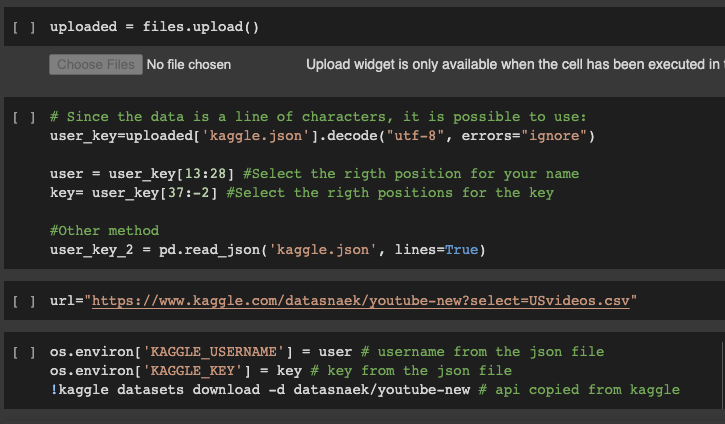
\includegraphics[width=13cm]{kaggle_upload.png}
\end{figure}


\subsection{Carga de datos}
Una vez nos hemos descargado los datasets y los tenemos en nuestro cloud, vamos a descomprimir el fichero y cargar los distintos datasets en un array de datasets que contendr\'a los diferentes datasets de cada mercado.
\begin{figure}[h!]
\centering
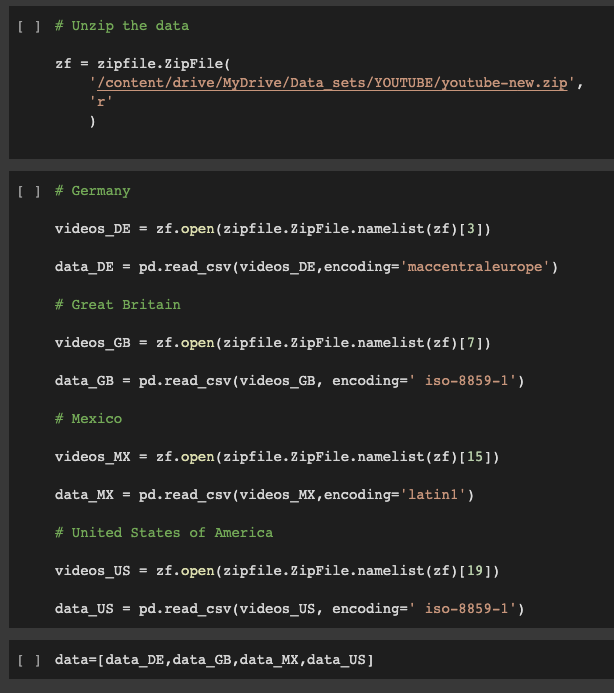
\includegraphics[width=13cm]{data_load.png}
\end{figure}



\subsection{Selecci\'on datos}
Primero de todo vamos a eliminar las filas con valores True en los atributos l\'ogicos ya que son minor\'ia y no son estad\'isticas que nos interesen para nuestro analisis.
\begin{figure}[h!]
\centering
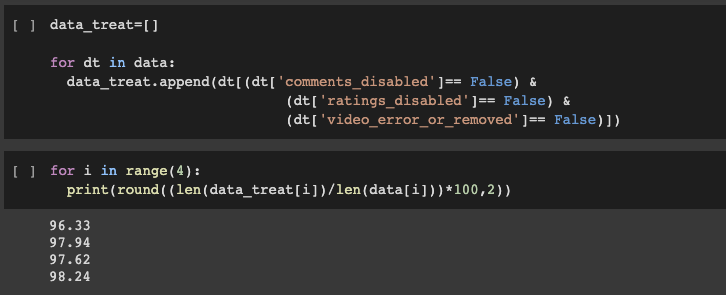
\includegraphics[width=13cm]{data_selection_1.png}
\end{figure}



Como podemos ver, eliminando estas columnas mantenemos el 96 porciento de los datos.

Debido a que ya solo nos quedan valores verdaderos para esas 3 columnas (comments{\textunderscore}disabled, ratings{\textunderscore}disabled y video{\textunderscore}error{\textunderscore}or{\textunderscore}removed), vamos a eliminarlas.
\begin{figure}[h!]
\centering
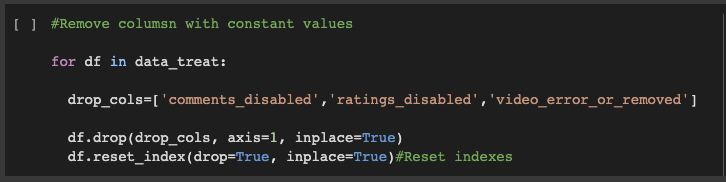
\includegraphics[width=13cm]{data_selection_2.png}
\end{figure}


\subsection{Eliminamos categor\'ia sin informaci\'on (category = 29)}

No existe informaci\'on sobre que categir\'ia representa el id 29, por lo tanto eliminamos \'esta del dataset. Otra raz\'on para eliminarla es que al no saber que representa dicha categor\'ia, aun en el caso que pudi\'esemos extraer alguna informaci\'on para la categor\'ia 29, no podr\'iamos darle un sentido concreto

A\'un eliminandola, preservamos el 95 porciento de la informaci\'on.

\begin{figure}[h!]
\centering
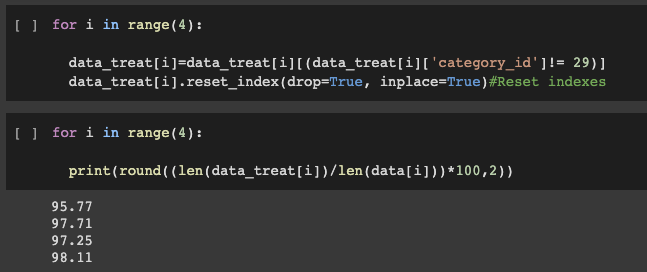
\includegraphics[width=13cm]{remove_category.png}
\end{figure}

\subsection{Correcci\'on  trending date}

Los formatos en los que las fechas nos vienen dadas, no son consistentes entre ellos. Por lo tanto, vamos a transformar todas las columnas que contengan un valor de fecha a tipo datetime, empezando por la columna trending date.

\begin{figure}[h!]
 \centering
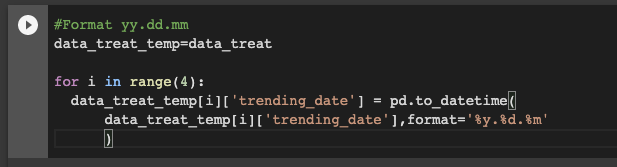
\includegraphics[width=13cm]{correc_trending.png}
\end{figure}

\subsection{Correcci\'on  publish time}
Vamos a realizar la misma operaci\'on con la columna publish time.

\begin{figure}[h!]
\centering
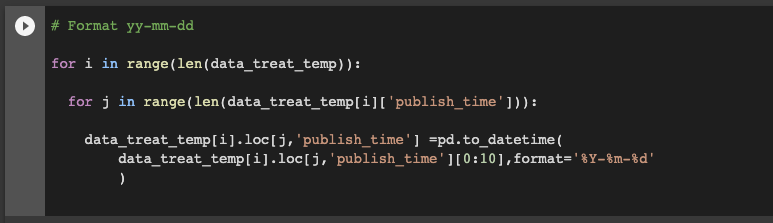
\includegraphics[width=13cm]{correc_publish.png}
\end{figure}

\subsection{Correcci\'on  textos}
La parte de language cleaning ees una de las m\'as importantes para nuestro proyecto ya que tener textos limpios y analizables sirve como una muy buena fundaci\'on para proyectos de an\'alisis futuros.


En nuestro caso hemos definido diferentes funciones para corregir caracteres mal codificados que hemos aplicado a las columnas: title, channel{\textunderscore}title,  tags y description.

\begin{figure}[h!]
\centering
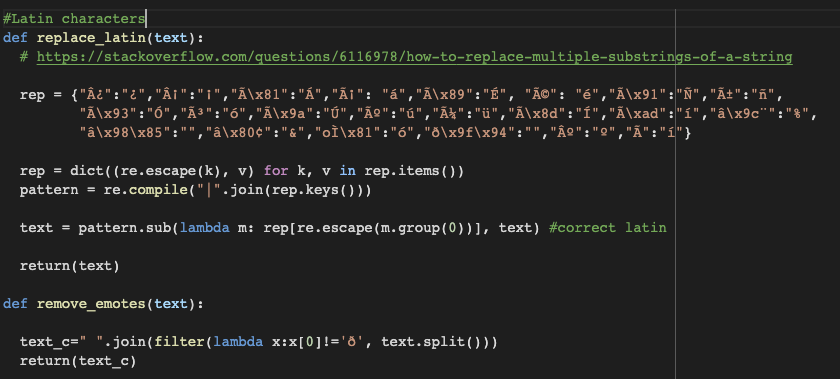
\includegraphics[width=13cm]{latin_characters.png}
\end{figure}

\begin{figure}[h!]
\centering
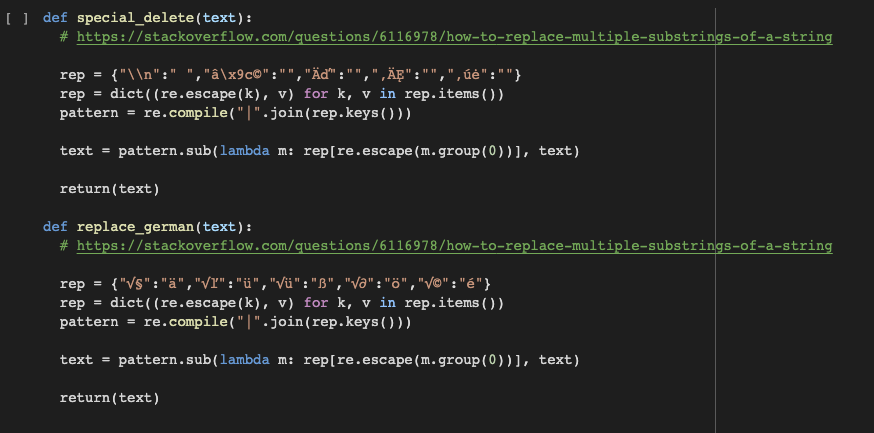
\includegraphics[width=13cm]{german_characters.png}
\end{figure}


\begin{figure}[h!]
\centering
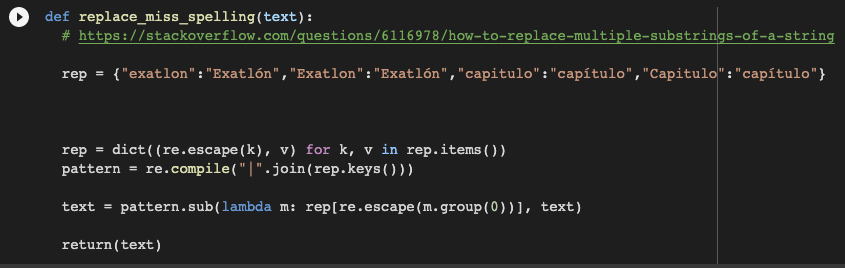
\includegraphics[width=13cm]{misspellings.png}
\end{figure}

\'Estas funciones se aplican a cada uno de los datasets para poder limpiar las columnas correctamente.

\section[item_metricas]{Generaci\'on de m\'etricas y an\'alisis de datos}

Es complicado analizar nuestros datos ya que no tenemos forma de saber si un video puede ser un outlier, por ejemplo tenemos videos con un gran n\'umero de visitas pero pocos comentarios (lo que llamariamos un click bait), o un video con pocas visitas pero un gran n\'umero de comentarios.
\\
Para poder analizar estos sucesos vamos a crear una serie de m\'etricas que nos ayudar\'an a realizar an\'alisis m\'as concretos sobre los v\'ideos.

\subsection{Generaci\'on m\'etrica video sentiment}
La metrica relative video sentiment (o rvs) se calcula utilizando la f\'ormula {\itshape (likes-dislikes)/sum(likes+dislikes)} y nos ayudar\'a a hacernos una idea de el sentimiento que genera un video sobre 1.

\begin{figure}[h!]
\centering
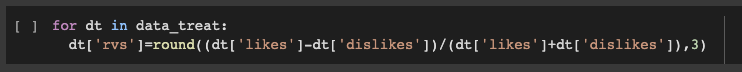
\includegraphics[width=13cm]{rvs_gen.png}
\end{figure}

Haciendo un plot de las frecuencias obtenidas sobre esta m\'etrica, nos damos cuenta de que los videos que llegan a ser Trend, tienden a tener un ratio de likes/dislikes de un 75 porciento.
\begin{figure}[h!]
\centering
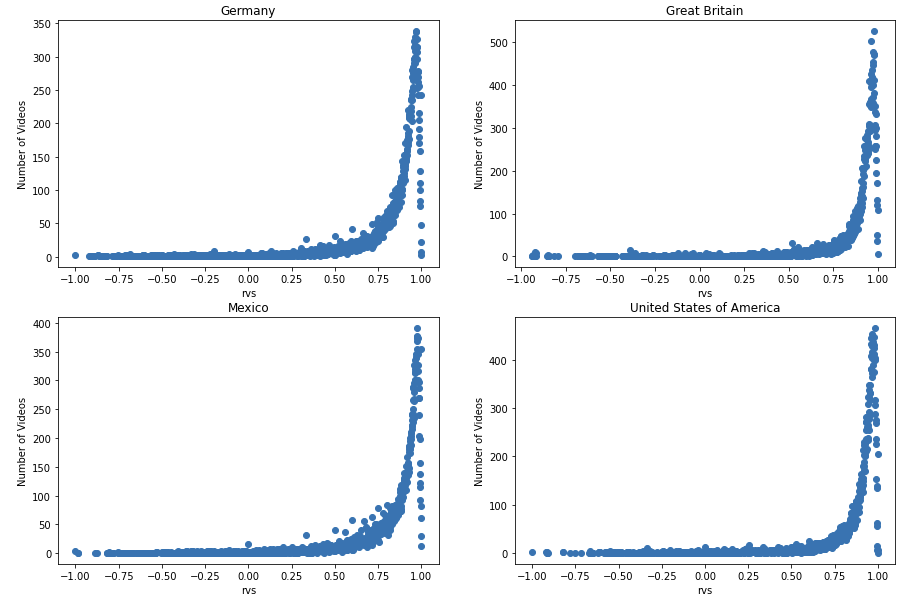
\includegraphics[width=14cm]{rvs_plot.png}
\end{figure}

\subsection{Generaci\'on m\'etrica relevancia}
Sabemos que para los usuarios comentar un video conlleva m\'as esfuerzo que darle a like o a dislike. Tambi\'en entendemos que un video tiene mayor cantidad de comentarios cuando los viewers tienen algo que decir sobre el tema o alg\'un comentario a provocado controversia.

Para medir esto, hemos creado un atributo rel{\textunderscore}elevance, el cual se calcula con la formula {\itshape comment{\textunderscore}count/(likes+dislikes)}. Cuando su valor tiende a 1 asumimos que el video es relevante para los viewers y cuando es mayor que 1 quiere decir que es muy relevante.
\begin{figure}[h!]
\centering
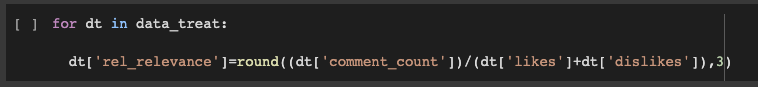
\includegraphics[width=13cm]{rel_gen.png}
\end{figure}

Haciendo un plot de las frecuencias de este valor, podemos observar que la mayor parte de los videos tiene un valor menor que  1.  De hecho, observamos que los videos que alcanzan Trending tienen a tener un ratio menor que 0.5, alcanzando un pico claro en 0.25.

Esto nos da a entender que los videos que alcanzan Trending no suelen ser muy pol\'emicos en general, lo cual tiene sentido ya que suelen ser videos que atraen a un p\'ublico general.

\begin{figure}[h!]
\centering
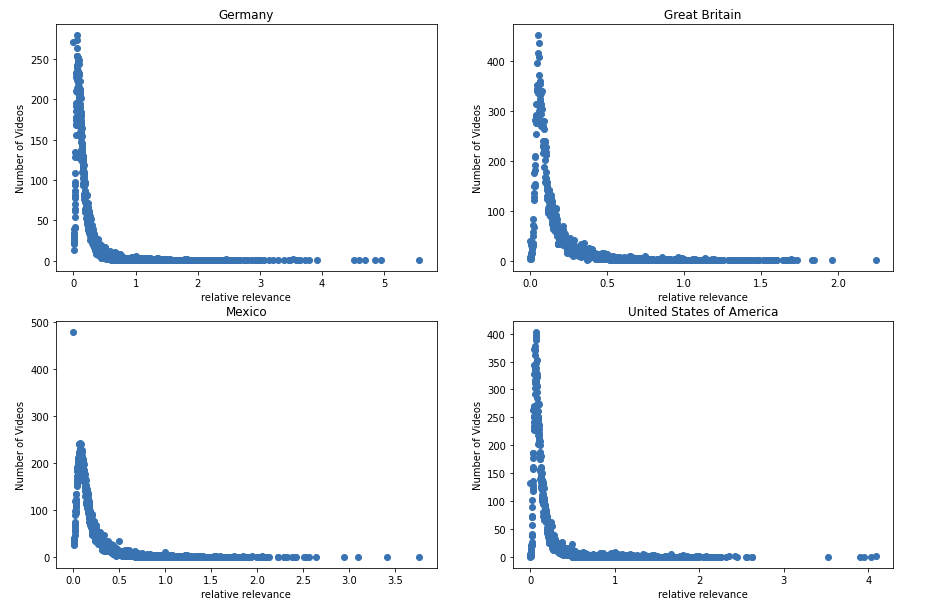
\includegraphics[width=14cm]{rel_relevance_plot.png}
\end{figure}

\subsection{Generaci\'on m\'etrica sentiment engagement}
Por \'ultimo vamos a generar 3 atributos relacionados con el sentiment engagement de los videos, \'estos ser\'an el positive engagement, negative engagement y overall engagement.

El positive engagement se calcular\'a utilizando la f\'ormula: {\itshape likes/views}

\begin{figure}[h!]
\centering
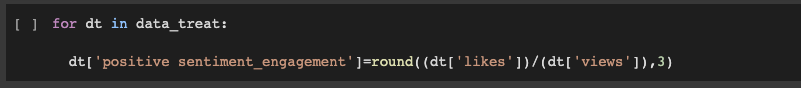
\includegraphics[width=13cm]{pos_eng_gen.png}
\end{figure}

El negative engagement se calcular\'a utilizando la f\'ormula: {\itshape dislikes/views}

\begin{figure}[h!]
\centering
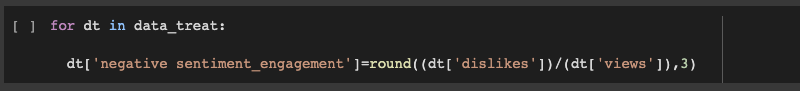
\includegraphics[width=13cm]{neg_eng_gen.png}
\end{figure}

El overall engagement se calcular\'a utilizando la f\'ormula: {\itshape (likes-dislikes)/views}

\begin{figure}[h!]
\centering
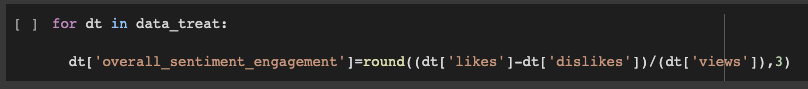
\includegraphics[width=13cm]{ove_eng_gen.png}
\end{figure}

Realizando un plot de las frecuencias, es f\'acil darse cuenta de que la tendencia en todos los pa\'ises es que m\'as de el 75\% de los videos est\'n en un rango de [0-10\%] rvs (likes-dislikes) por visualizaci\'on del video.

\begin{figure}[h!]
\centering
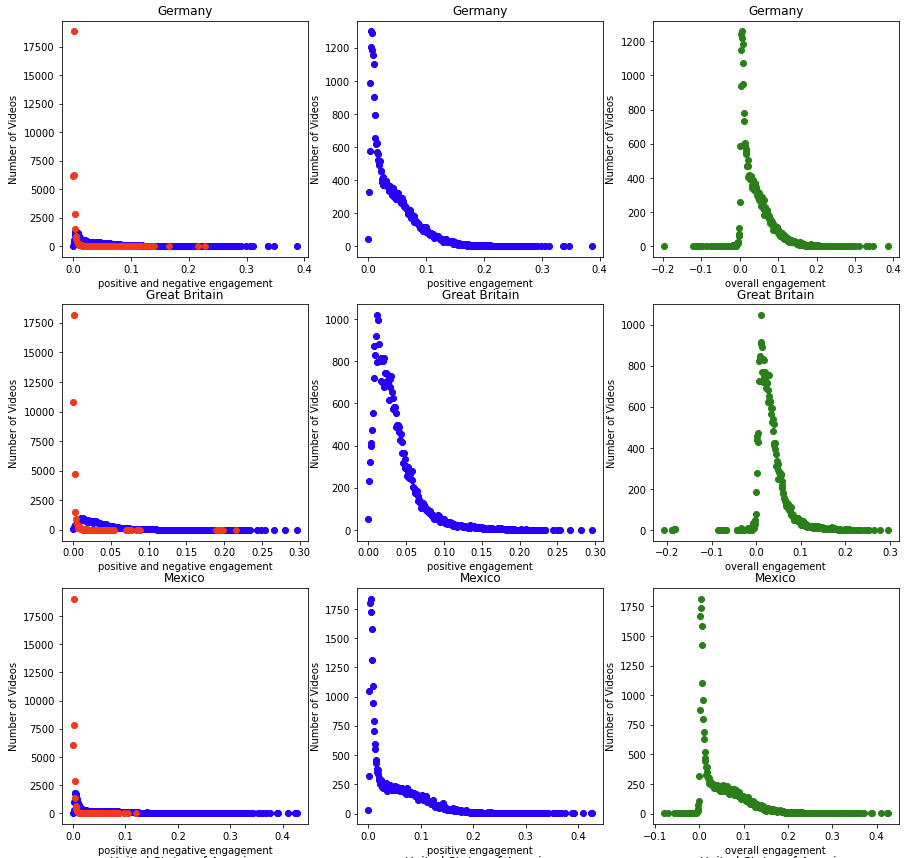
\includegraphics[width=13cm]{engagement_1.png}
\end{figure}

\begin{figure}[h!]
\centering
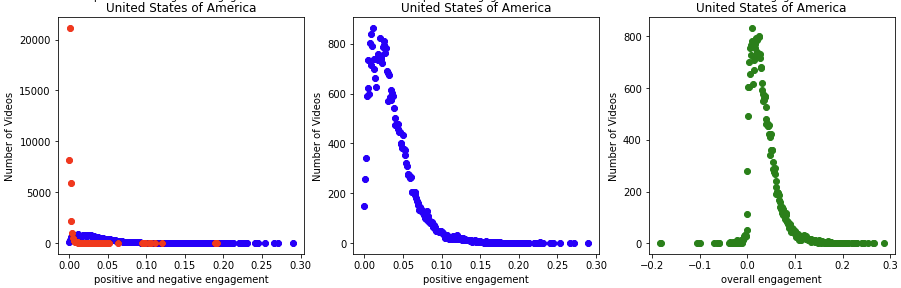
\includegraphics[width=13cm]{engagement_2.png}
\end{figure}

\subsection{Comprobaci\'on de normalidad}

Nuestro daset presenta dos dificultades a la hora de comprobar si los datos y las m\'etricas sigen una distribuci\'on normal. Por una parte el gran n\'umero de datos hace inviable la aplicaci\'on del test de normalidad de {\itshape  Shapiro Wilk}, por otra parte, al existir muchos valores repetidos para un atributo el test de {\itshape Anderson Darling} no es fiable ya que siempre devolver\'a como resultado el rechazo de la hip\'otesis nula. Por este motivo nos centramos en los valores de {\itshape Kurosis} y {\itshape Skewness}. Para estos test, t\'ipicamnete se considera que una distribuci\'on es normal cuando el valor de {\itshape Kurtosis} est\'a entre $-2$ y $+2$ y para {\itshape skewness} los valores deben caer dentro del intervalo entre $-0.8$ y $+0.8$.

Podemos comprobar que tanto los valores de los datos en crudo, como las m\'etricas que hemos implementado no siguen una distribuci\'on normal. Con el fin de solucionar este problema y conseguir una distribuci\'on homogenea de la varianza, hemos optado por utilizar en primera instancia una transformaci\'on de {\itshape Yeo Jhonson}, puesto que nos permite aplicar el mismo c\'odigo sobre todos los atributos (una transformaci\'on de {\itshape Yeo Jhonson} a diferencia de {\itshape Boxcox} nos permite trabajar con valores negativos y ceros).

\begin{verbatim}
# transform and save data &  lambda value 

fitted_data = []
fitted_lambda = {}

names=['views','likes','dislikes','comment_count','rvs','rel_relevance','overall_sentiment_engagement']
names_fitted=['fviews','flikes','fdislikes','fcomment_count','frvs','frel_rel','foverall_sen_eng']
country=['Germany','Great Britain','Mexico','United States of America']

for j,odata in enumerate(original_data):

  lambda_list= []

  for i,col in enumerate(names):
    
    fdata, lambda_val = stats.yeojohnson(odata.loc[:,col])

    odata[names_fitted[i]]=fdata
    lambda_list.append(lambda_val)
  
  fitted_lambda[country[j]]=lambda_list

\end{verbatim}

Hemos creado una funci\'on {\itshape normal check} que nos devuelve 1 cuando los datos de un atributo siguen una distribuci\'on normal (en las condiciones especificadas arriba) y 0 cuando no la sigue. La hemos aplicado sobre todas las columnas de todas los datasets y los datos los hemos visualizado como un dataframe que se copia abajo:

\begin{figure}
\centering
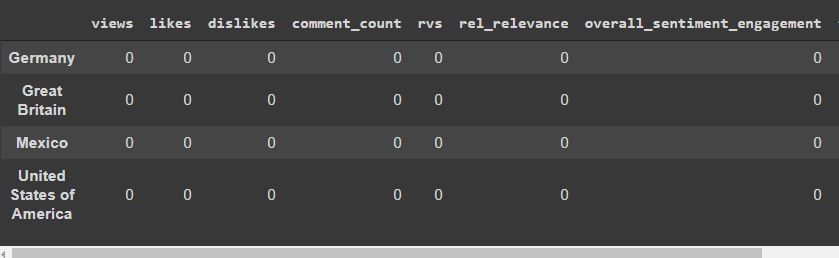
\includegraphics[width=12cm]{dataframe_1.JPG}
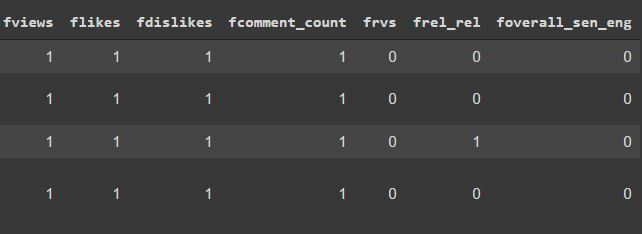
\includegraphics[width=12cm]{dataframe_2.JPG}
\end{figure}
 
Como se puede ver los datos en crudo se han podido transformar de forma que ahora siguen una distribuci\'on normal, pero las m\'etricas no siguen todav\'ia una distribuci\'on normal.

Con el fin de corregir este hecho hemos realizado una transformaci\'on por quantiles sobre las m\'etricas  y obtenido los siguientes resultados.

\begin{figure}[h!]
\centering
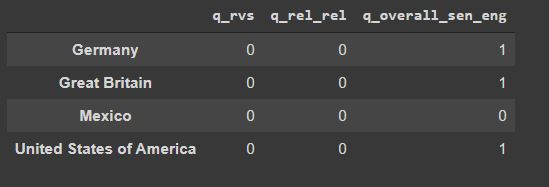
\includegraphics[width=12cm]{dataframe_3.JPG}
\end{figure}

Con el fin de comprobar la discrepancia presente en los datos de {\itshape M\'exico} hemos hecho una representaci\'on de densidades para la los datos {\itshape q\_overall\_sen\_eng}, es decir los datos que cuya variable  ha sufrido una transformaci\'on por quantiles.

\begin{figure}[h!]
\centering
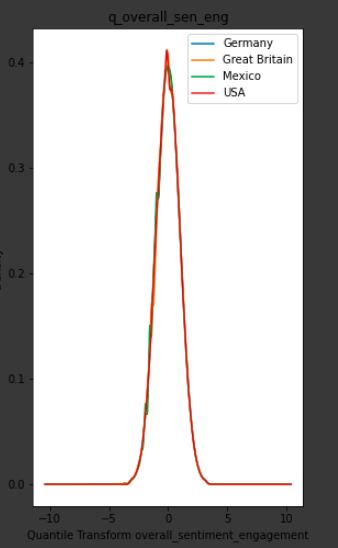
\includegraphics[width=5cm]{grafica_transformada.JPG}
\end{figure}

En esta curva no podemos apreciar ninguna diferencia significativa entre las curvas para cada pa\'is.

En conclusi\'on ahora contamos con los datos transformados en crudo v\'ia {\itshape Yeo\-Jhonson} que siguen una distribuci\'on normal y la m\'etrica {\itshape overall\_sent\_eng} que transformada por quartiles tambi\'en sige una distribuci\'on normal por lo que podremos aplicar test de correlaci\'on, modelos de regresi\'on y otros test estad\'isticos para m\'etricos.

\section[item_pruebas]{Pruebas estad\'isticas}
\subsection{Cu\'ales son las 50 palabras m\'as populares por pa\'is y atributo}

Una de las formas que tenemos de seguir o analizar tendencias en videos de YouTube, es contar las palabras en los diferentes atributos de los videos.

En nuestro caso, vamos a contar las palabras en los titulos de los videos, comentarios, descripciones y canales.

Para empezar vamos a cargar los datos con los textos ya transformados y limpios.
\\
\\
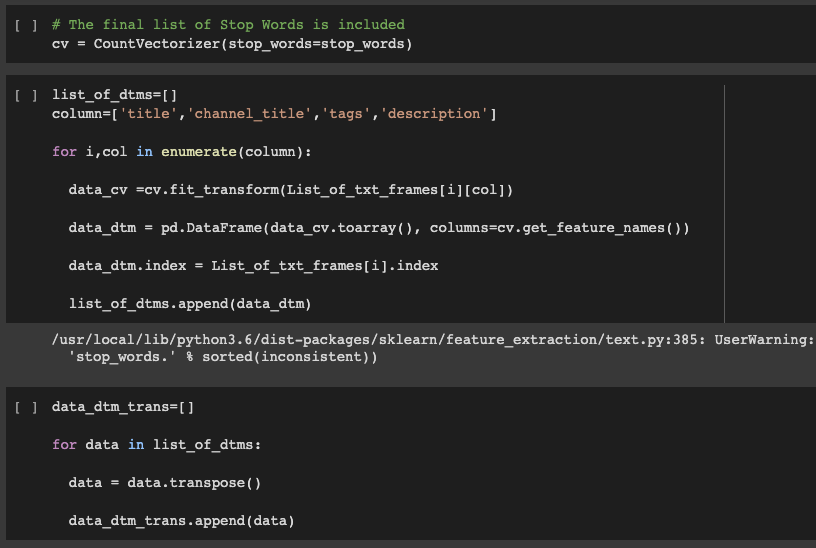
\includegraphics[width=13cm]{50_words_1.png}
\\

Una vez tenemos los datos cargados, vamos a encontrar las 50 palabras mas populares para cada atributo del video.

\begin{figure}[h!]
\centering
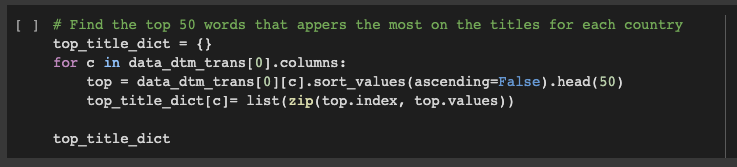
\includegraphics[width=12cm]{50_words_title.png}
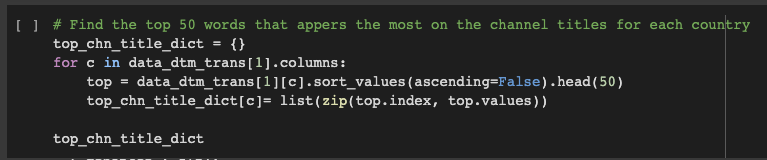
\includegraphics[width=12cm]{50_words_channel.png}
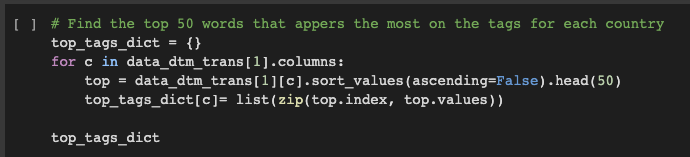
\includegraphics[width=12cm]{50_words_tags.png}
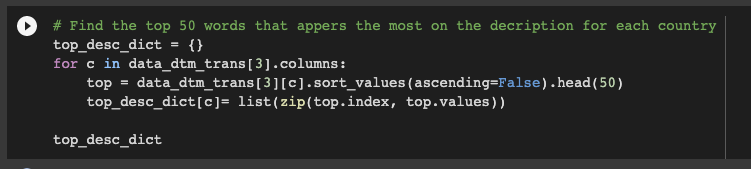
\includegraphics[width=12cm]{50_words_desc.png}
\end{figure}

Por \'ultimo, vamos a realizar un wordcloud de los datos obtenidos.

Empezamos con los wordcloud de las tags.

Como podemos ver,  en alemania hay varias palabras en turco, esto se debe a la gran inmigraci\'on Turca que existe en el pais. Esto provoca que los datos est\'en divididos en turco y alem\'an.
\\
\\
El resto de wordclouds son bastante claros, a destacar en el Mejicano, que podemos ver la TV Azteca y exatlon, que es un programa de gran \'exito en el pais.
\\
\\
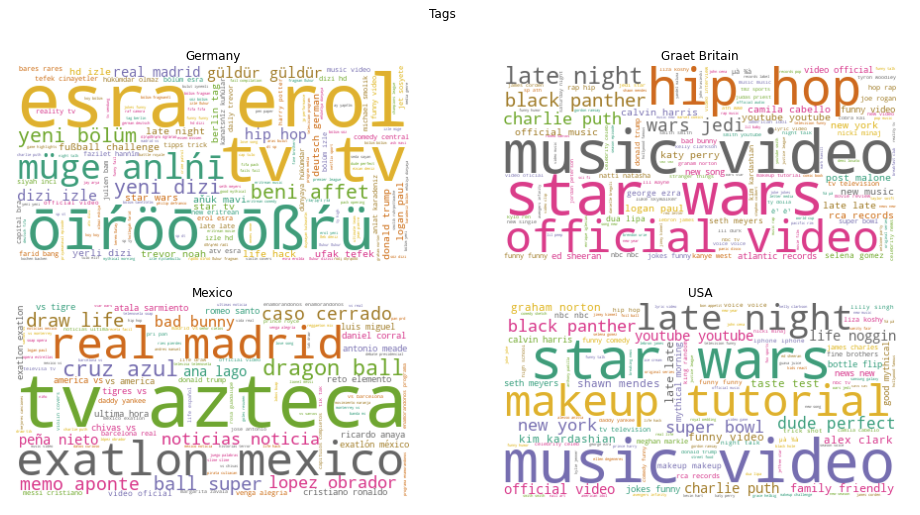
\includegraphics[width=13cm]{wordcloud_tags.png}
\\
\\
A continuaci\'on mostraremos el wordcloud de los t\'itulos de los videos.
\\
\\
A destacar que la palabra trump aparece m\'as en Alemania que en EEUU. Los videos musicales parecen ser muy populares. Los videos de f\'utbol y otros deportes son mucho mas populares en M\'ejico que en el resto de pa\'ises. Los vengadores y Star Wars tienen bastante impacto en UK y EEUU.
\\
\\
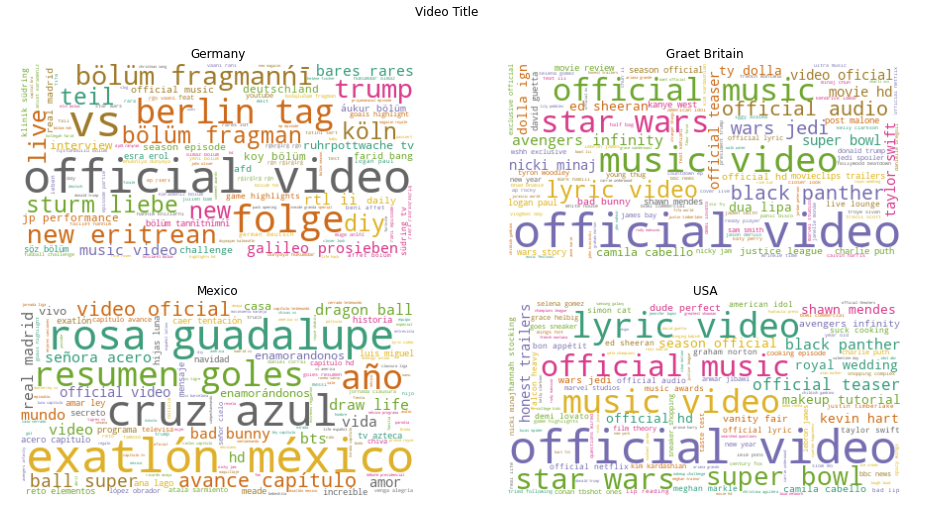
\includegraphics[width=13cm]{wordcloud_title.png}
\\
\\
Por \'ultimo vamos a mostrar las palabras mas utilizadas en las descripciones de los videos.
Como se puede observar, lo que mas se ven son nombres de redes sociales y webs, esto se debe a que la mayor\'ia de creadores de contenido introducen sus redes sociales en la descripci\'on. Para poder obtener informaci\'on relevante de \'esta wordcloud necesitamos realizar m\'as tareas de limpieza.
\\
\\
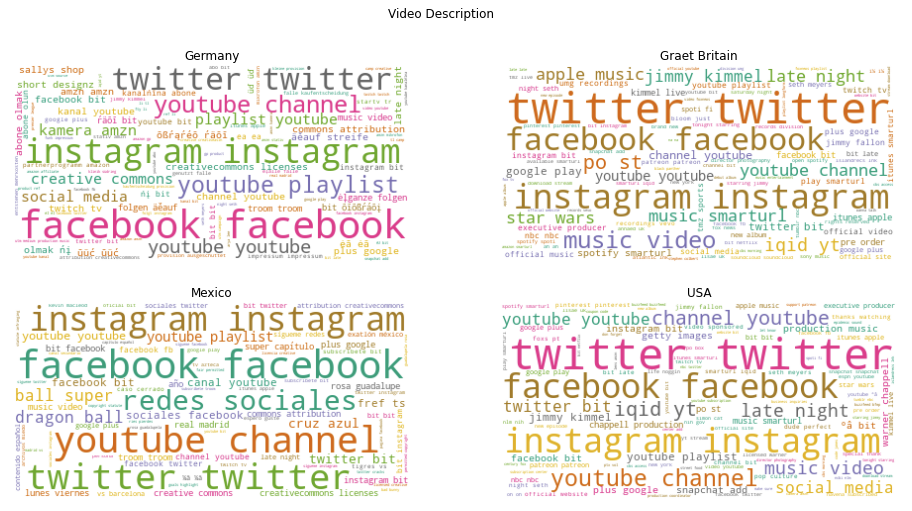
\includegraphics[width=13cm]{wordcould_desc.png}

\subsection{Cu\'anto tarda un video en llegar a Trending}
Para analizar cu\'anto tarda un video en llegar a Trending, vamos a generar una nueva columna con este valor, que calcularemos restando la fecha de Trending con la fecha de publicaci\'on.
\\
\\
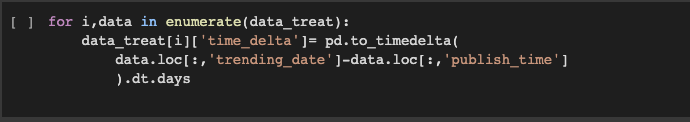
\includegraphics[width=13cm]{time_delta_gen.png}
\\
\\
Una vez tenemos estos datos, vamos a realizar un plot de frecuencias para el n\'umero de videos por dias que tarda en llegar a trending.
\\
\\ 
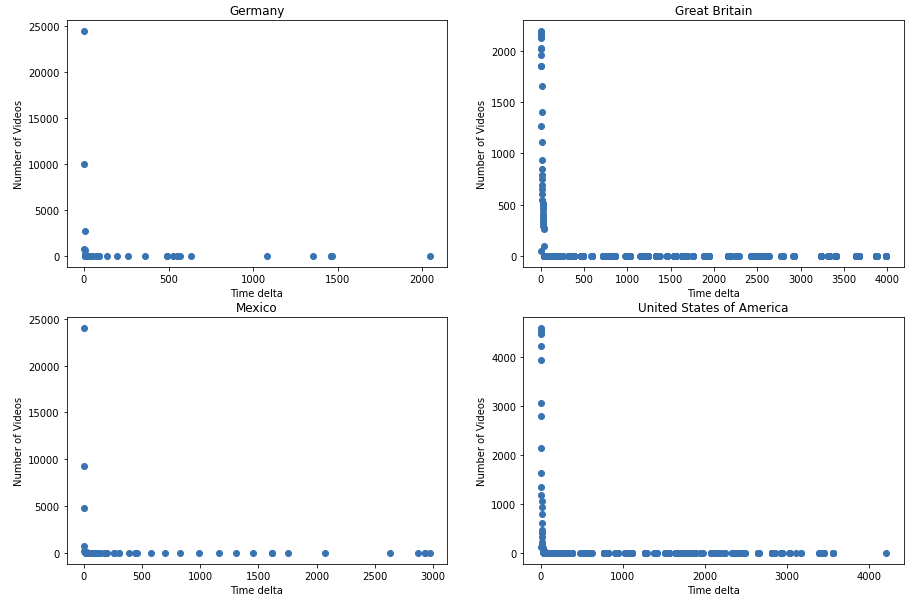
\includegraphics[width=13cm]{plot_freq_times.png}
\\
\\
Con estas gr\'aficas podemos ver que la mayor\'ia de videos llegan a trending en los primeros d\'ias tras su lanzamiento. Para hacernos una mejor idea vamos a realizar un plot de que porcentajes de videos llegan a trending en diferentes rangos de tiempo.
\\
\\ 
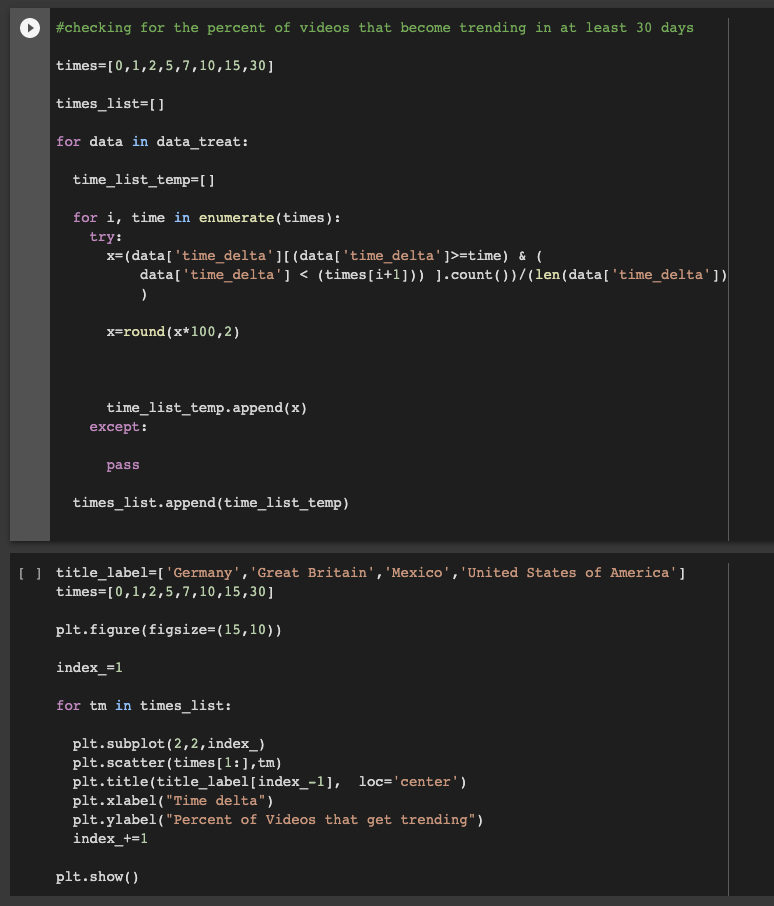
\includegraphics[width=13cm]{plot_freq_code.png}
\\
\\ 
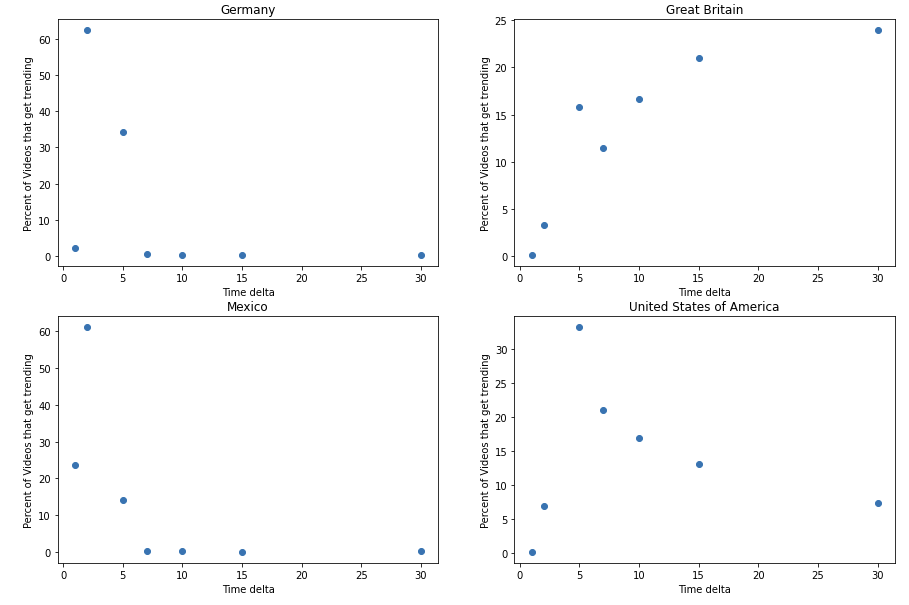
\includegraphics[width=13cm]{plot_freq_perc.png}
\\
\\
Los datos mostrados representan un 98\% de los videos. Estos resultados son muy interesantes ya que nos dan una idea de cuando tarda algo en hacerse popular en un los diferentes paises, cada cuanto utilizan la plataforma los usuarios en los diferentes paises, o cuanto tarda un usuario en ver algo fuera de sus intereses habituales.
\subsection{Qu\'e categor\'ias tienen m\'as \'exito en cada pa\'is}

Para realizar visualizaciones correctas sobre las categorias de los videos, vamos crear una columna con el nombre de la categor\'ia del video (ahora mismo solo teniamos sus ids).
\\
\\
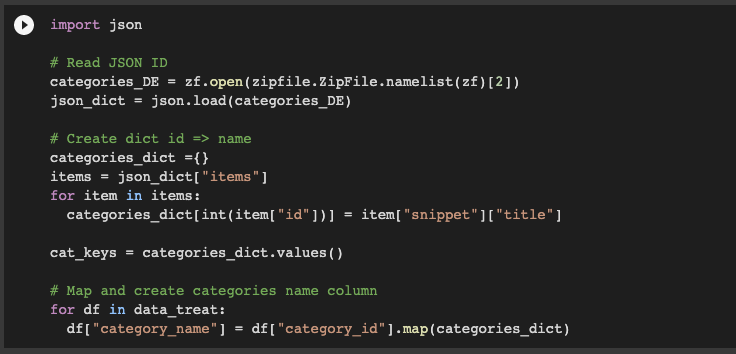
\includegraphics[width=13cm]{categories_1.png}
\\
\\
Una vez tenemos la columna creada, vamos a obtener el numero total de videos en trending por categoria en cada mercado.
\\
\\
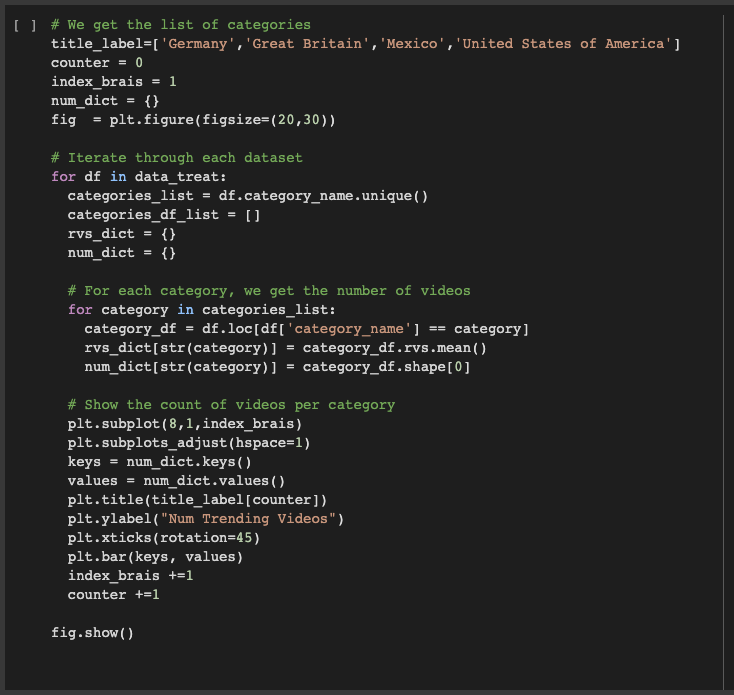
\includegraphics[width=13cm]{categories_2.png}
\\
\\
Con este plot vamos a ser capaces de ver la distribucion de las vistas por cada categoria. Como datos mas relevantes que se pueden observar, los videos de categor\'ia entretenimiento son los que suelen alcanzar trending con m\'as asiduidad.
\\
\\
Otro dato que me ha parecido muy interesante es como los videos musicales son muy populares en EEUU y UK, mientras que en Mejico o Alemania no son casi relevantes.\'Esta informaci\'on podr\'ia ser de gran utilidad para artistas que intentan crecer en diferentes regiones o mercados.
\\
\\
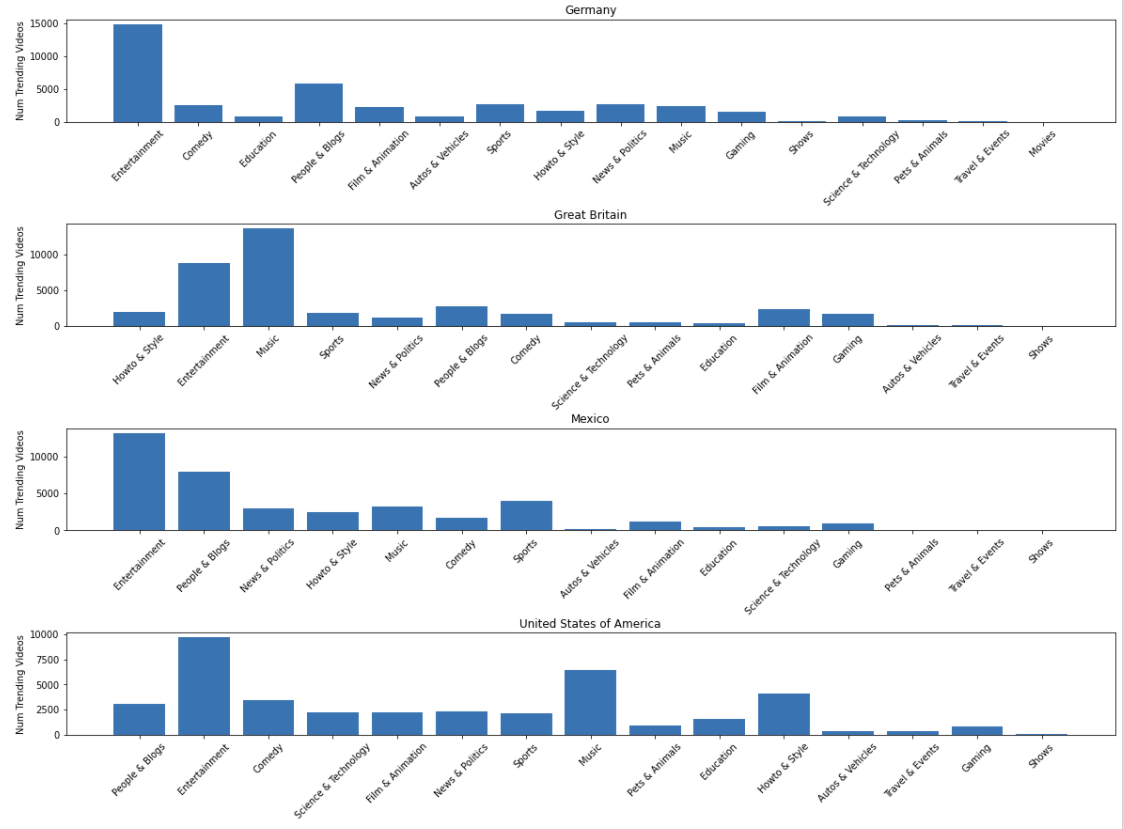
\includegraphics[width=13cm]{plot_categories.png}

\subsection{Modelo de Regresi\'on}
\'Esta secci\'on se ha realizado en R a diferencia de el resto de la pra\'actica que est\'a desarrollada en Python.



\section[item_conclusiones]{Conclusiones}
Hemos obtenido m\'ultiples conclusiones muy interesantes, hemos visto c\'omo los diferentes pa\'ises interact\'uan con los videos, ya sea desde el punto de vista de como reaccionan a ellos o cu\'ales son los m\'as populares.
\\
\\
Todas estas conclusiones ser\'an de gran utilidad para cualquier creador de contenido que trate de hacerse un hueco en YouTube, o incluso grandes empresas que quieran realizar propuestas de marketing a trav\'es de la plataforma podri\'ian utilizar \'esta informaci\'on para especializar los anuncios por comunidad o mercado.


\begin{thebibliography}{9}

\bibitem{td1} Leonard Berzkowitz,%
	\emph{ Advances in Experimental Social Psychology}, 1967,  Academic press
\bibitem{td2} Richard McElreath, Robert Boyd,%
	\emph{ Mathematical Models of Social Evolution: A Guide for the Perplexed}, 2007, The University of Chicago Press
\bibitem{td3}Thomas L. Saaty and Joyce M. Alexander,%
	\emph{Thinking with models: Mathematical Models in the Physical, Biological, and Social Sciences}, 2015, RWS Publications
\bibitem{dd1}Jason Radford and Kenneth Joseph,%
	\emph{Theory In, Theory Out: The Uses of Social Theory in Machine Learning for Social Science}, 2020, doi.org/10.3389/fdata.2020.00018

\end{thebibliography}

\end{document}
